\chapter{Get Started with Elmer}

\section{Introduction}

Getting started using \texttt{Elmer} should be a smooth and easy process.  Beginners at all levels may have issues with getting started and that can be a barrier to the use of  \texttt{Elmer}.  This chapter is meant to provide help to beginners, to make it easy to start using \texttt{Elmer} and \texttt{ElmerGUI}.\\

A typical use case would be for someone with a particular application in mind that wants to find out whether \texttt{Elmer} is a suitable choice.  Being able to quickly download and run an Elmer tutorial should make the experience easy enough so the user gets an answer in a short amount of time.

\chapter{Windows -- Download}

This chapter will discuss installing Elmer in Windows.  Windows 10 is used for these instructions.  The steps should also work with earlier versions of Windows, as long as they are 64 bits.

\section{Download Elmer}

To download the most recent release of Elmer, go to the following website:\\

\url{https://www.nic.funet.fi/pub/sci/physics/elmer/}

\begin{figure}[H]
\centering
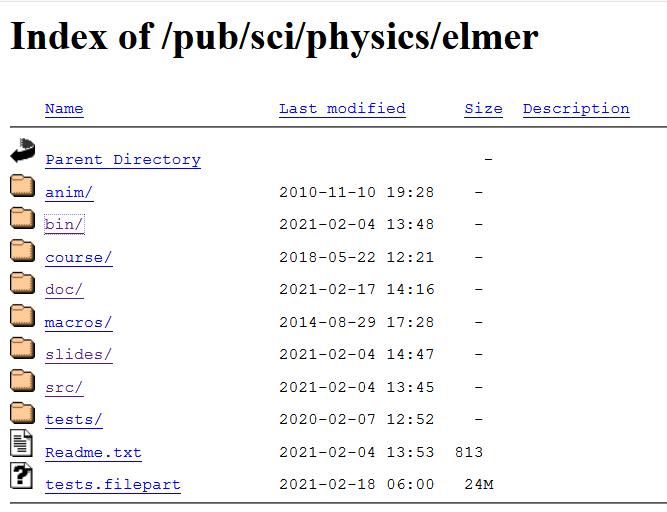
\includegraphics[width=0.8\textwidth]{elmer}
\caption{Elmer Bin Windows}\label{fg:elmer}
\end{figure}

Once on that page, there are several folders to notice, such as `bin', `doc', `slides', and `tests', as shown in Figure~\ref{fg:elmer}.  To download Elmer, click on `bin' and then `windows', and the list of Elmer installers will appear, as shown in Figure~\ref{fg:elmer-bin-win}.

\begin{figure}[H]
\centering
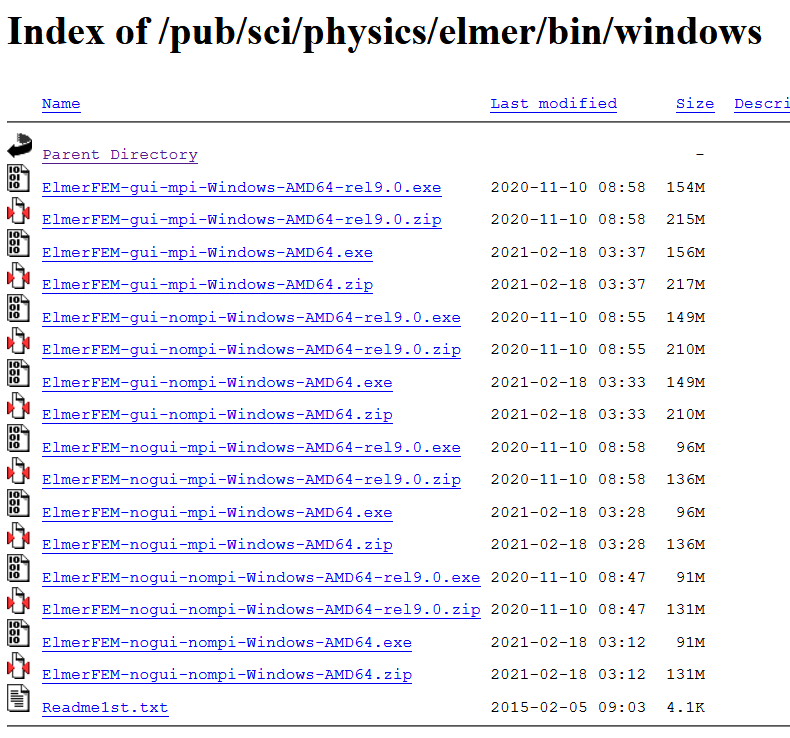
\includegraphics[width=0.9\textwidth]{elmer-bin-win}
\caption{Elmer Installers}\label{fg:elmer-bin-win}
\end{figure}

There four main categories to select from, such as `gui-mpi', `gui-nompi', `nogui-mpi', and `nogui-nompi'.  There also some labelled with `rel9.0', which are builds of the most recent official release and should be considered as the stable builds.  The other files not labelled with `rel9.0', are the nightly builds and are the most recent builds.\\

For the first time installing Elmer in Windows, it is recommended to select `gui-nompi', and `rel9.0'.  The files with .exe extension are an installer for Windows, which is what is recommended.  So out of the entire list, we want to download this file:\\

\texttt{ElmerFEM-gui-nompi-Windows-AMD64-rel9.0.exe}

\section{Download Elmer Documentation}

Return to this page, this time select `doc' for the most recent documentation for Elmer:\\

\url{https://www.nic.funet.fi/pub/sci/physics/elmer/}

\begin{figure}[H]
\centering
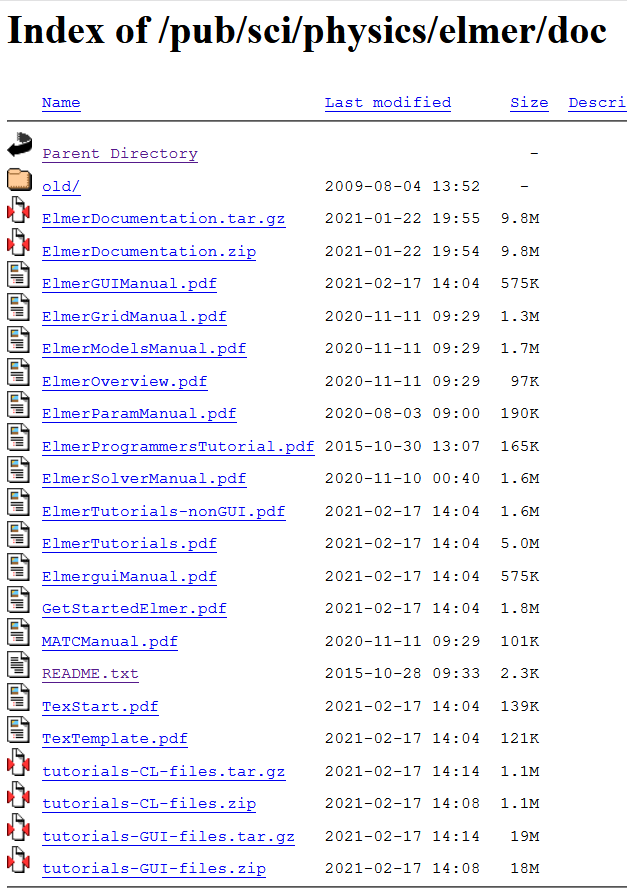
\includegraphics[width=0.8\textwidth]{elmer-doc}
\caption{Elmer Doc}\label{fg:elmer-doc}
\end{figure}

Download the individual files to get the most recent build of the manuals.  Be sure to download `ElmerTutorials' for the ElmerGUI tutorials, `ElmerGUI Manual' for instructions about ElmerGUI, and `ElmerSolverManual', which describes each solver in detail.\\

Also be sure to download the file, `tutorials-GUI-files.zip', because this zipped folder contains working examples of ElmerGUI projects, one for each tutorial.

\newpage

\section{Download Paraview}

Since we are taking care of downloads, let's go ahead and get Paraview.  It's not really needed to get started with Elmer and ElmerGUI, but you'll need it at some point in the near future.  Download Paraview now, but don't install it just yet.  We'll cover installation of Paraview a little later in this discussion.\\

Go to the Download section of the Paraview website:\\

 \url{https://www.paraview.org/download/}\\

Select one of the top items, in particular a file ending in .exe, so you will download a Windows installer version.  You should now have a file like this:\\

\texttt{ParaView-5.9.0-RC3-Windows-Python3.8-msvc2017-64bit.exe}\\

On the Paraview download page, there are several other files, such as `getting started', `tutorial', that would be very useful to download.  This would be a good opportunity to download the instructions for Paraview.


\chapter{Windows -- Install}

\section{Install Elmer}

Navigate to the folder containing the Elmer installer and the documentation zip file.  Extract the zip file to a suitable folder.  Double click on the Elmer installer .exe file.  The installation process should look like figures~\ref{fg:installer-1}  through figure~\ref{fg:installer-10} on the following pages.  

\begin{figure}[H]
\begin{center}
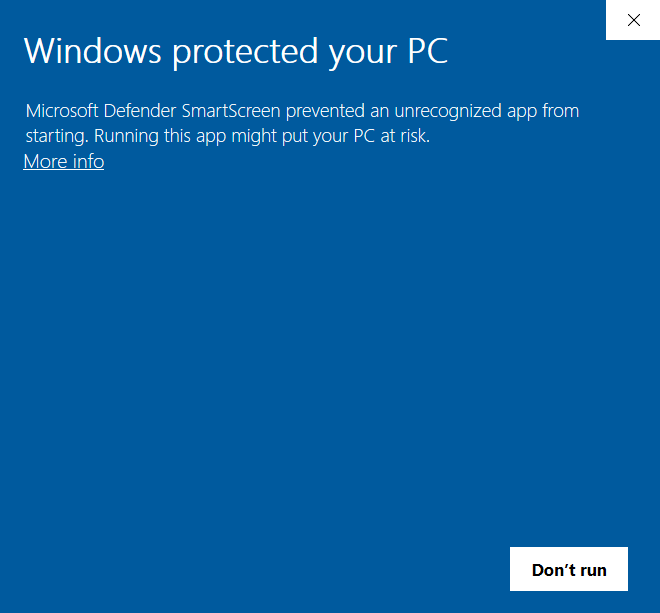
\includegraphics[width=0.48\textwidth]{installer-1}
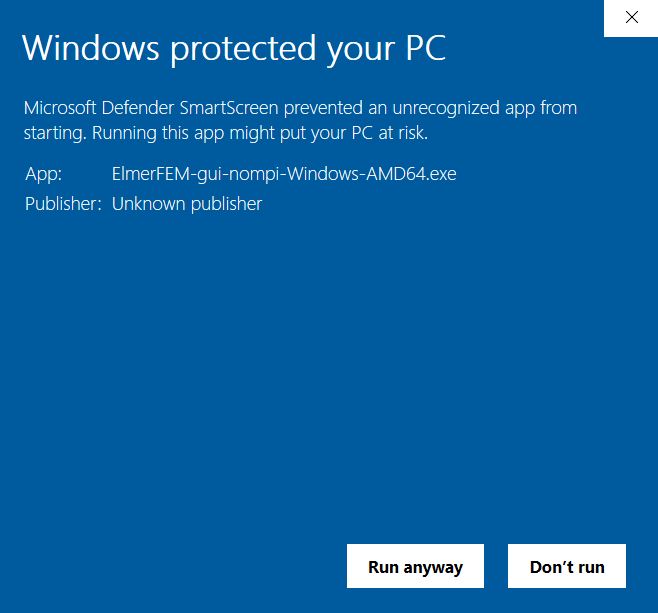
\includegraphics[width=0.48\textwidth]{installer-2}
\caption{Elmer installation, click on the More info button, then Run anyway}\label{fg:installer-1}
\end{center}
\end{figure}

You may get a blue screen while beginning the installation.  The first blue screen has a small button, `More info', that you must click on to get the second blue screen, where you will click on `Run anyway'. \\

From there just take the default actions up until you reach `Install Options', where you have a chance to select adding the path to Elmer.  Be sure to click on `Add Elmer...', either for all users or for current user.  If you aren't sure, pick `for current user'.  Also put a check into the check box for `Create Elmer Desktop Icon'.  From here, take the defaults and it should properly install Elmer.

\begin{figure}[H]
\begin{center}
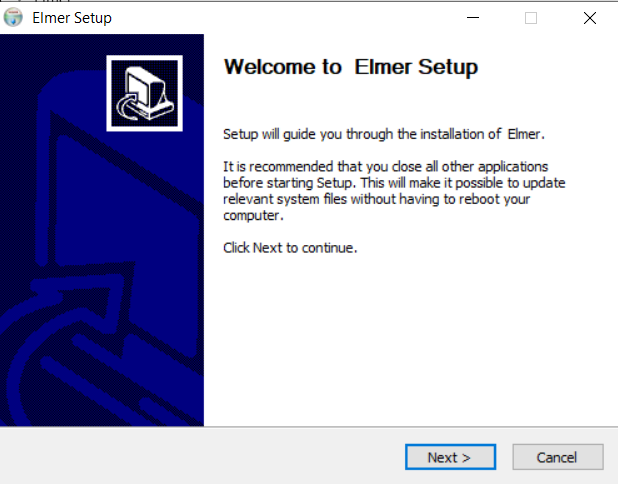
\includegraphics[width=0.48\textwidth]{installer-3}
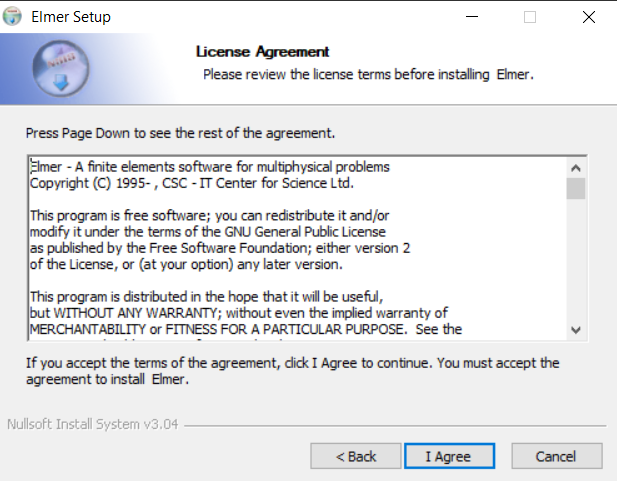
\includegraphics[width=0.48\textwidth]{installer-4}
\caption{Elmer installation}\label{fg:installer-3}
\end{center}
\end{figure}

\begin{figure}[H]
\begin{center}
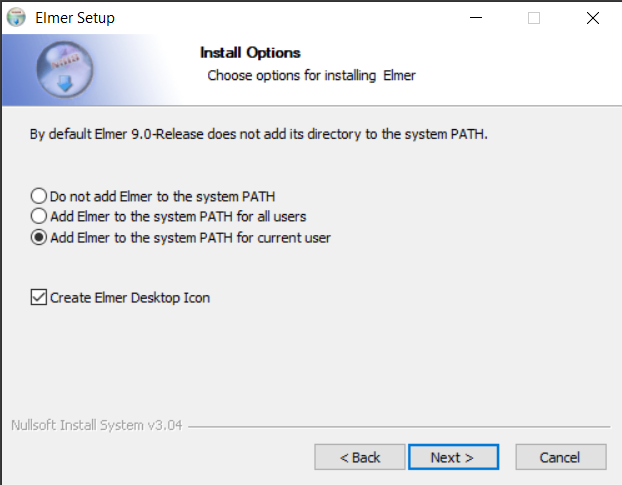
\includegraphics[width=0.48\textwidth]{installer-5}
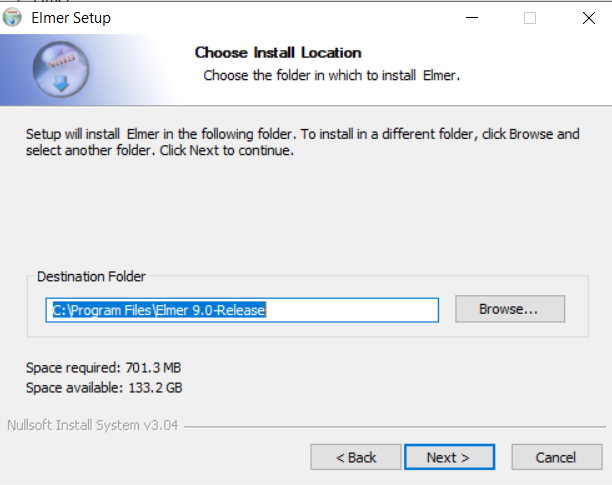
\includegraphics[width=0.48\textwidth]{installer-6}
\caption{Select Install Option: Add Elmer to the system PATH for current user}\label{fg:installer-5}
\end{center}
\end{figure}

\begin{figure}[H]
\begin{center}
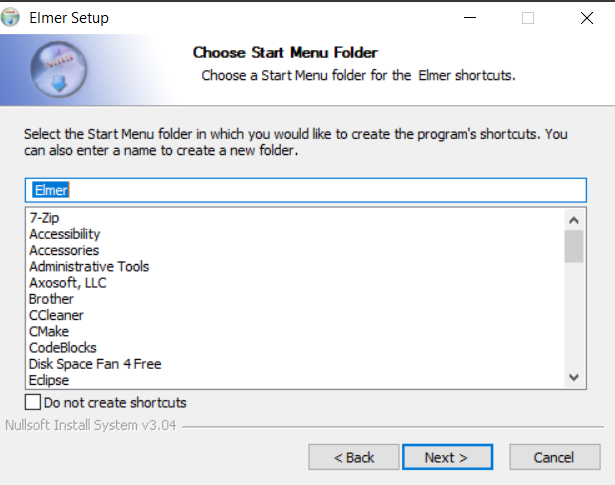
\includegraphics[width=0.48\textwidth]{installer-7}
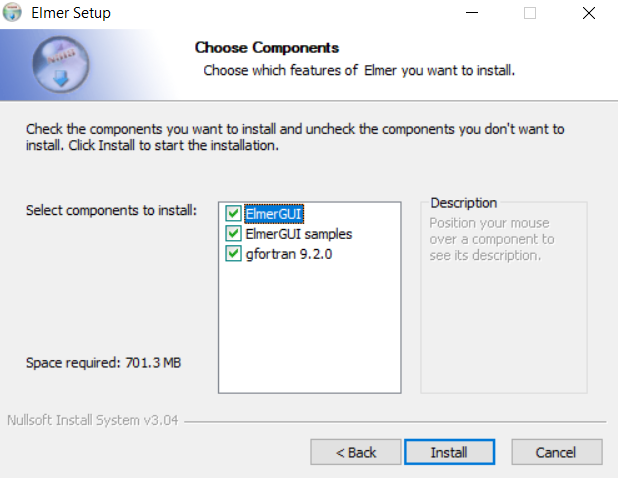
\includegraphics[width=0.48\textwidth]{installer-8}
\caption{Elmer installation}\label{fg:installer-7}
\end{center}
\end{figure}

\begin{figure}[H]
\begin{center}
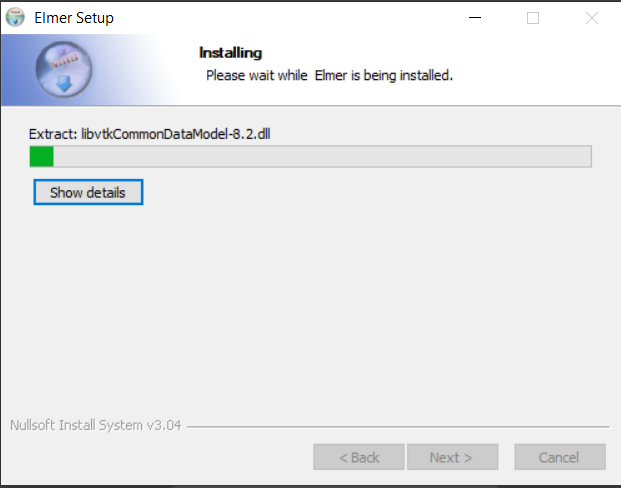
\includegraphics[width=0.4\textwidth]{installer-9}
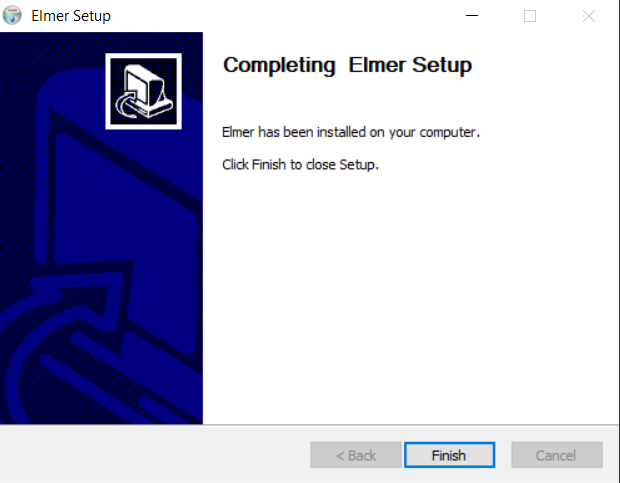
\includegraphics[width=0.4\textwidth]{installer-10}
\caption{Elmer installation}\label{fg:installer-9}
\end{center}
\end{figure}

After the installation process has finished, you should see an icon on the desktop for ElmerGUI.  Go ahead and double click on the icon to start ElmerGUI.  Please refer to the ElmerGUI manual for instructions on using ElmerGUI, and try out the first tutorial. 

Since Paraview hasn't been installed yet, after loading the first tutorial  if you click on the little RGB flag icon in the upper right of the menu bar to try and start Paraview, nothing much will happen.  If you hover the cursor over the flag after clicking on it, you will see in the lower left of the window the message `Unable to start Paraview'.  In the meantime, to start ElmerVTK click on the top menu bar icon `Run', then click on `Start ElmerVTK'.


\section{Install Paraview}

Navigate to the folder containing the Paraview installer.  Double click on the installer to start the installation process.  There really aren't any options that need to selected or changed for a successful installation.  The installer won't create a desktop icon, but will create an entry in the Start menu.\\

The installer will not add Paraview to the system path, so we will perform that step ourselves.


\chapter{Windows -- Add the path to Paraview}

\section{Path to Elmer}

If we set the path to Paraview, then ElmerGUI will be able to start Paraview from inside of ElmerGUI.  In other words, with a proper path setting, clicking on the ElmerGUI icon for Paraview, will start Paraview and load the current .vtu file, if it exists.

To set the path after installing Paraview, click on `Start', then `Settings'.  As shown in figure~\ref{fg:path-1}, start typing in the search box `environment', then select the result for `Edit environment variables for your account'.  

\begin{figure}[H]
\begin{center}
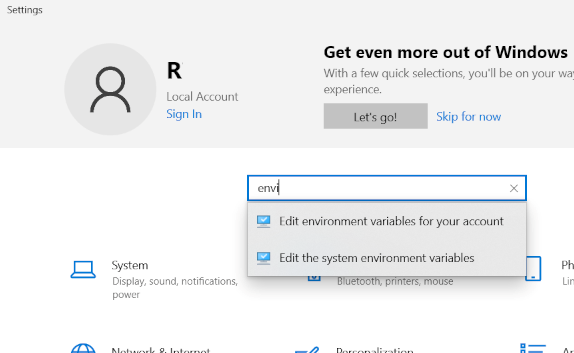
\includegraphics[width=0.95\textwidth]{path-1}
\caption{Settings: Search for Environment variables}\label{fg:path-1}
\end{center}
\end{figure}

\newpage

As part of the operation of the Elmer installer, the path to Elmer will be created.  Let's verify that the path to Elmer exists.  Open the window then select `path' and click `edit', as shown in figure~\ref{fg:path-2}.   Notice Elmer is at the bottom of the list, since it was the most recently installed program.  

\begin{figure}[H]
\begin{center}
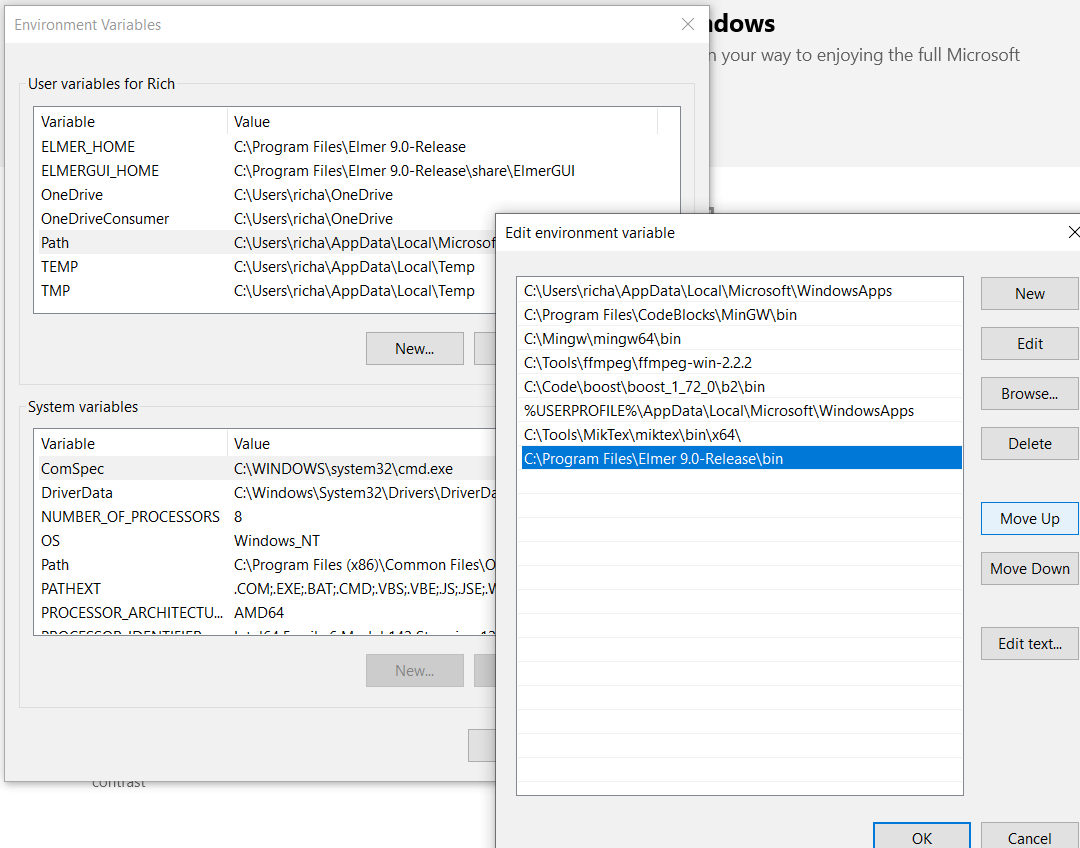
\includegraphics[width=0.9\textwidth]{path-2}
\caption{Path to Elmer installation}\label{fg:path-2}
\end{center}
\end{figure}

\section{Path to Paraview}

While you have the path variable open for editing, click on `new', and enter the path to Paraview.\\

One way to find out what is the exact path to your installation of Paraview is as follows.  Open File Explorer and select your system drive, such as C:, then open Program Files and then open the folder for Paraview.  Next open the bin folder and you will see an entry for Paraview.exe, this is the location that you want to enter into the path, as shown in figure~\ref{fg:path-3}.

\begin{figure}[H]
\begin{center}
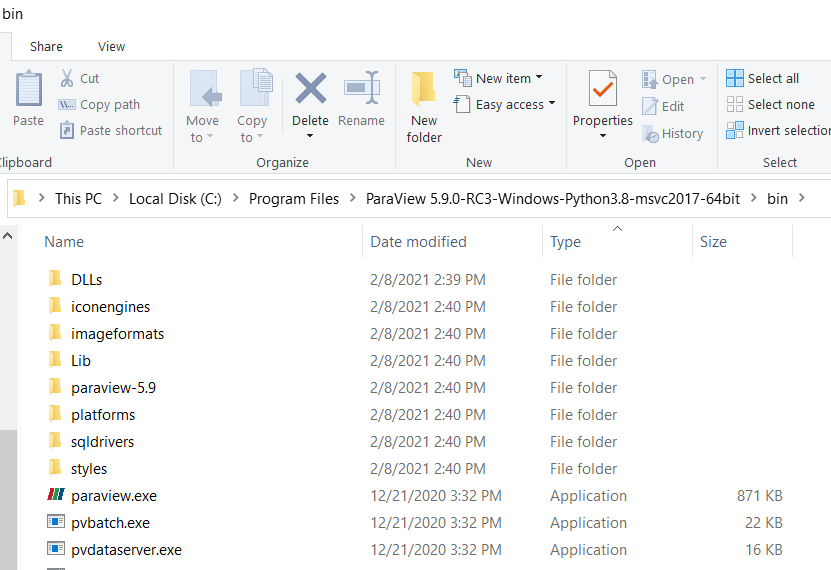
\includegraphics[width=0.75\textwidth]{path-3}
\caption{Select the path to Paraview}\label{fg:path-3}
\end{center}
\end{figure}

Copy the path to the bin folder into the new path environment variable.  Tip: you can actually copy and paste the path from File Explorer into the new environment path variable, as shown in figure~\ref{fg:path-4}.\\

\begin{figure}[H]
\begin{center}
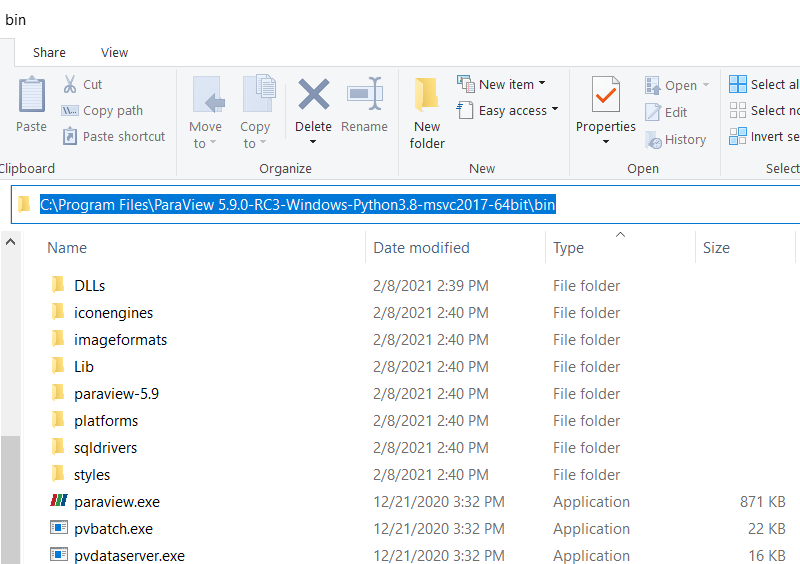
\includegraphics[width=0.75\textwidth]{path-4}
\caption{Copy the path to Paraview}\label{fg:path-4}
\end{center}
\end{figure}

Not completely necessary, but just suggested, you may want to move the path to 
Elmer up to the top of the list, as shown in figure~\ref{fg:path-5}.\\

Finally, move the entry for the path to Paraview up to just under the path to Elmer, as shown in figure~\ref{fg:path-5}.  Click `ok' to save your edits, then exit settings.

\begin{figure}[H]
\begin{center}
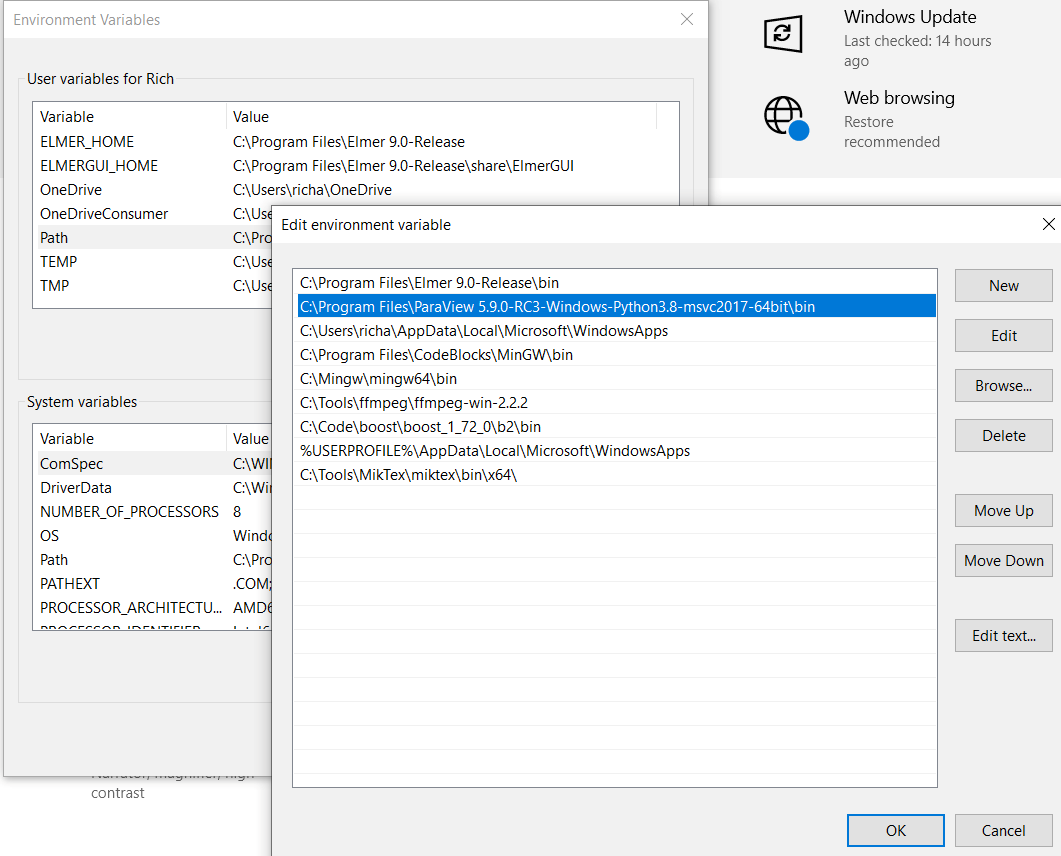
\includegraphics[width=0.9\textwidth]{path-5}
\caption{Create new path to Paraview}\label{fg:path-5}
\end{center}
\end{figure}

\section{Start Paraview from within ElmerGUI}

Open ElmerGUI, and click on the flag icon for Paraview, you should see a pop up window that says `Paraview Starting', followed by Paraview actually starting.  If you see an output window containing a red statement like `critical: In unknown, line 0', don't worry, it just means there wasn't a valid .vtu file found.  Run a tutorial, or find a valid .vtu file, and try again, Paraview should load the .vtu file and display a blank grey screen.

\chapter{Introduction to Paraview}

If you have loaded a valid Elmer .vtu file, upon opening Paraview you will see a blank grey screen, and many small icons, as shown in Figure~\ref{fg:para-2}.

\begin{figure}[H]
\begin{center}
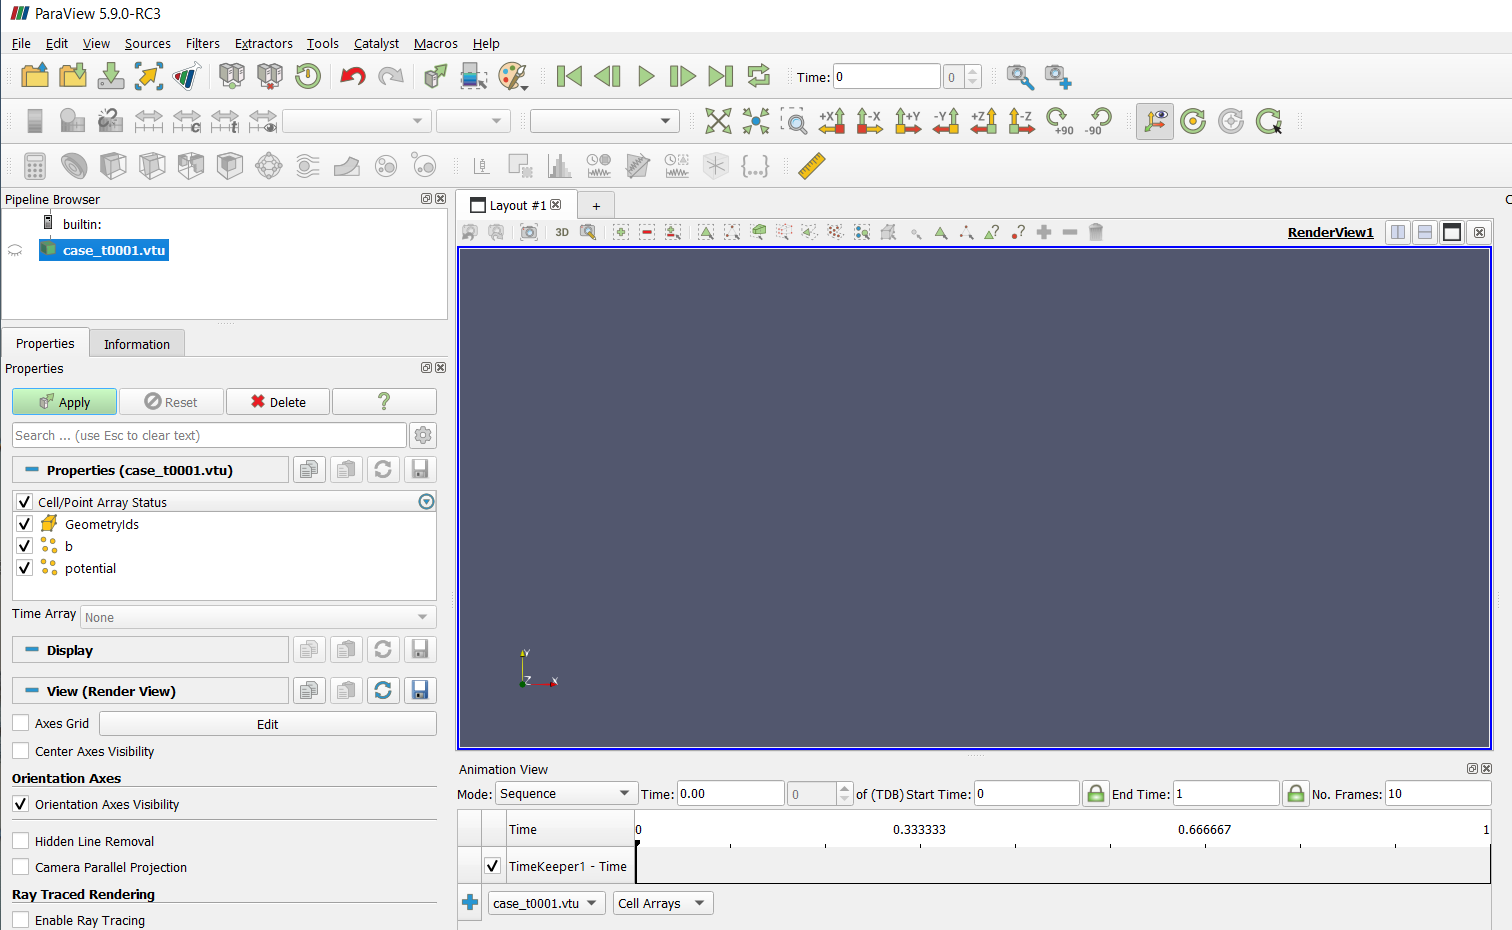
\includegraphics[width=0.58\textwidth]{para-2}
\caption{Initial Paraview screen}\label{fg:para-2}
\end{center}
\end{figure}

On the left side of the screen, as shown in Figure~\ref{fg:para-4}, near the middle is a light green button `Apply'.  Click on that button and the geometry will appear.

\begin{figure}[H]
\begin{center}
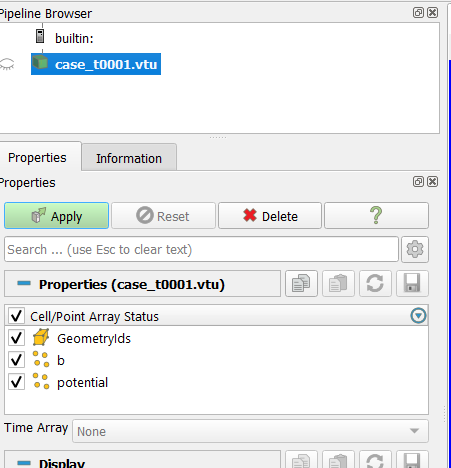
\includegraphics[width=0.38\textwidth]{para-3}
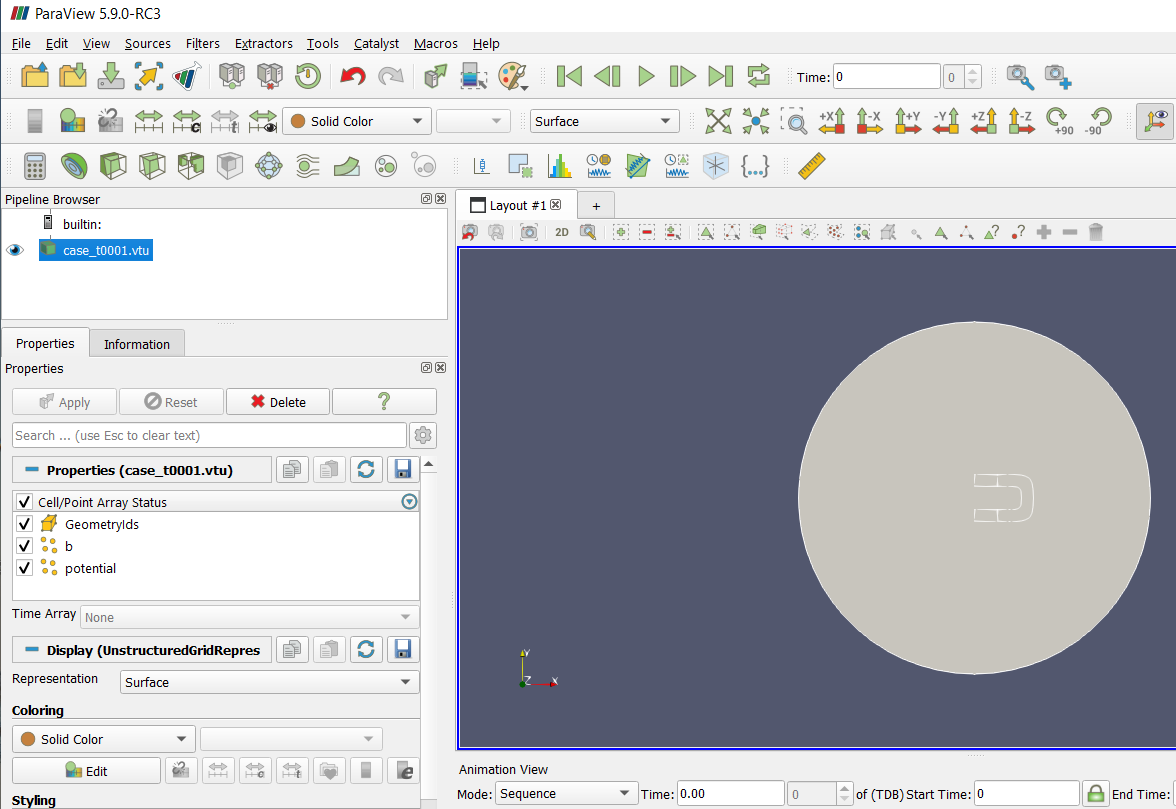
\includegraphics[width=0.57\textwidth]{para-4}
\caption{Left side click Apply, right side geometry appears}\label{fg:para-4}
\end{center}
\end{figure}

\newpage

Next, look on the left side below the window showing the variables, as shown in Figure~\ref{fg:para-5}, for a box labelled `Coloring'.  Click in that box for a drop down selection, pick `potential', then click `Apply'.  The potential will appear superimposed on the geometry, along with a color bar with the range of the potential.

\begin{figure}[H]
\begin{center}
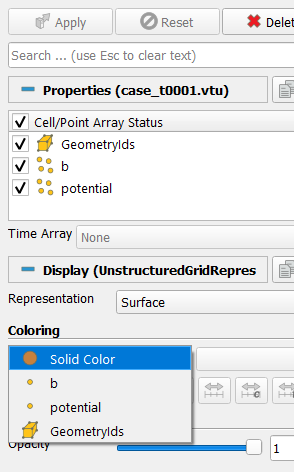
\includegraphics[width=0.3\textwidth]{para-5}
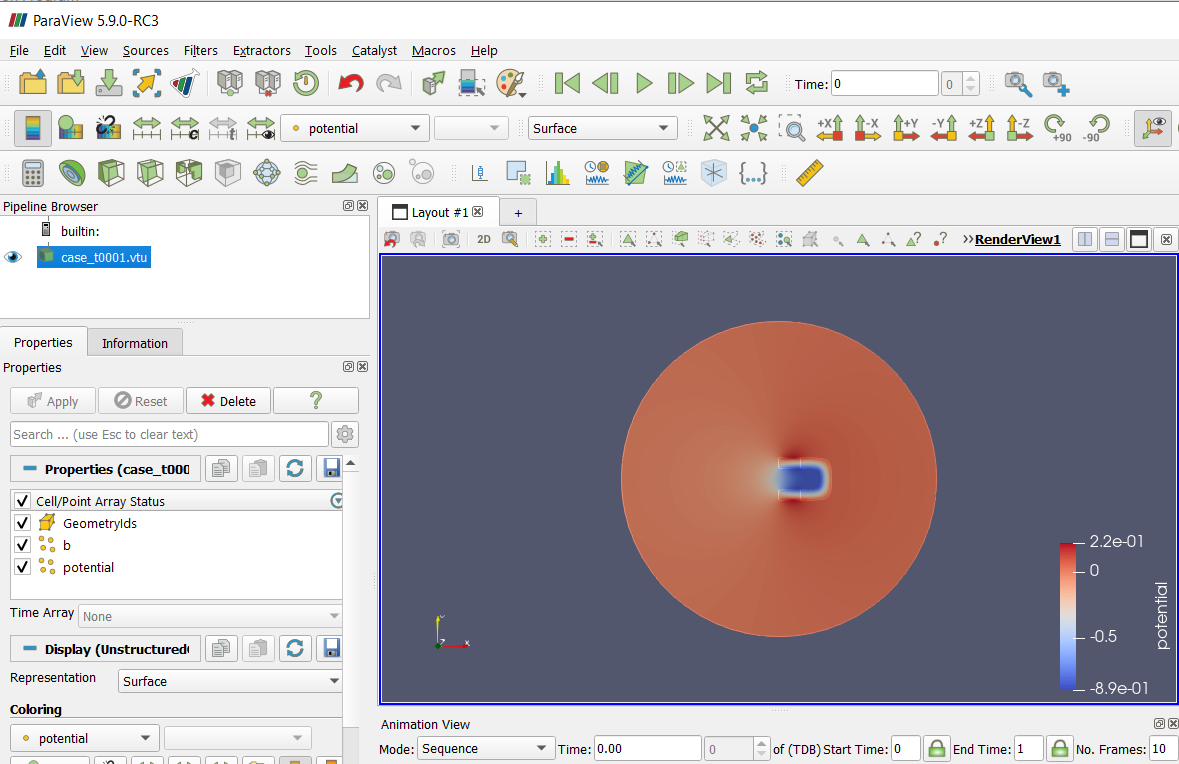
\includegraphics[width=0.68\textwidth]{para-6}
\caption{Initial Paraview screen}\label{fg:para-5}
\end{center}
\end{figure}

That is a very basic introduction to Paraview.  For more information, refer to the  Paraview website.

\chapter{Introduction to ElmerVTK}

ElmerGUI is equipped with ElmerVTK, a graphical post processor.  While ElmerVTK is not as powerful as Paraview, ElmerVTK is simpler to use.  After a successful ElmerSolver run, start ElmerVTK by clicking on `Run' on the top menu bar, then click on `Start ElmerVTK',  as shown in Figure~\ref{fg:vtk-1}.

\begin{figure}[H]
\begin{center}
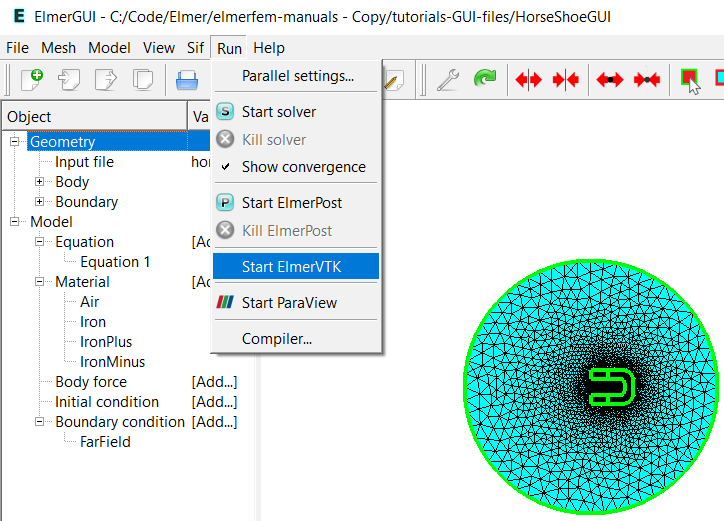
\includegraphics[width=0.8\textwidth]{vtk-1}
\caption{Start ElmerVTK}\label{fg:vtk-1}
\end{center}
\end{figure}

The ElmerVTK window will open, displaying the geometry,  as shown in Figure~\ref{fg:vtk-2}.  Click on the menu bar for the `Isocontours' menu.  In two places, variable and color, click for the drop down menu and select `potential'.

\begin{figure}[H]
\begin{center}
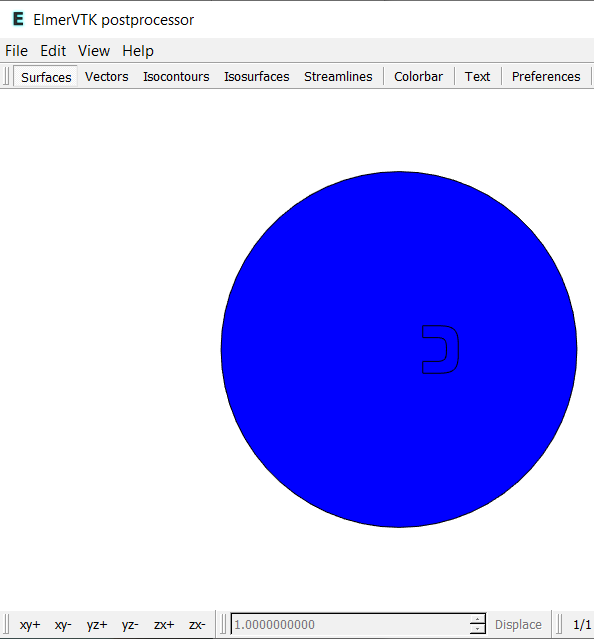
\includegraphics[width=0.45\textwidth]{vtk-2}
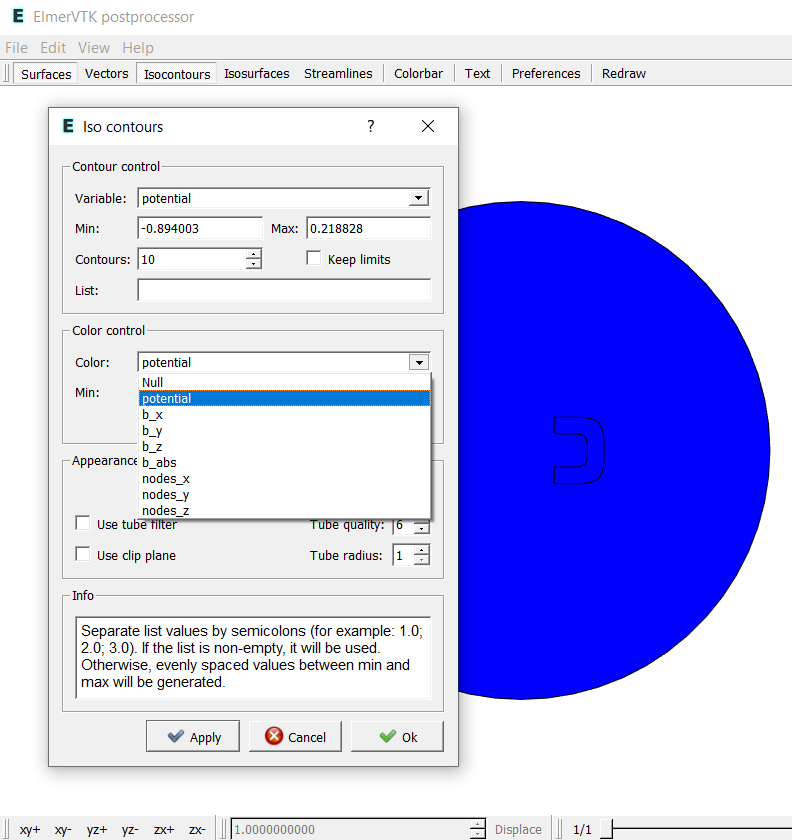
\includegraphics[width=0.45\textwidth]{vtk-3}
\caption{ElmerVTK showing geometry, select Isocontours}\label{fg:vtk-2}
\end{center}
\end{figure}

The isocontours of potential will show, superimposed on the geometry, as shown in Figure~\ref{fg:vtk-4}.  The number of isocontours look a little sparse, so open up the Isocontours menu again, and this time change number of `Contours' from 10 to 50.  That looks better.

\begin{figure}[H]
\begin{center}
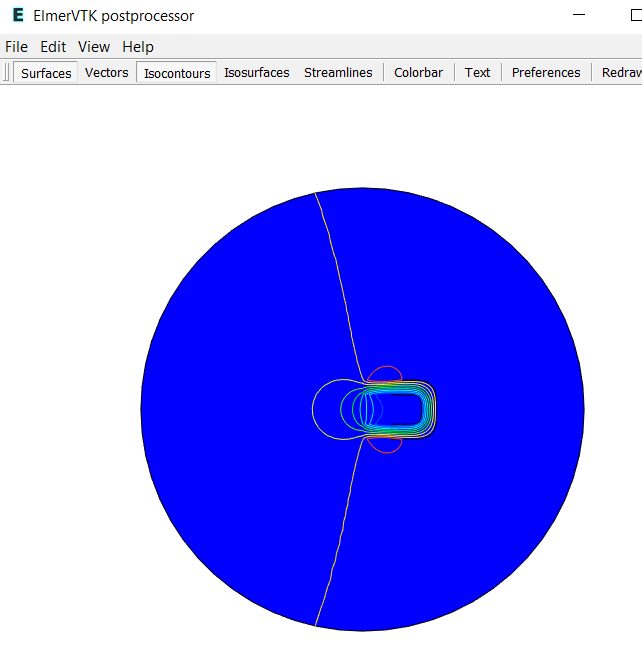
\includegraphics[width=0.48\textwidth]{vtk-4}
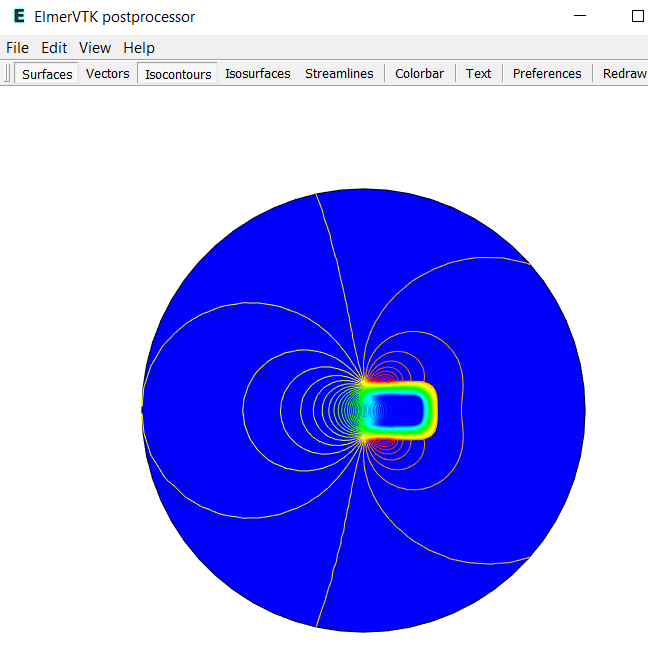
\includegraphics[width=0.48\textwidth]{vtk-5}
\caption{Isocontours of potential, 10 on left, 50 on right}\label{fg:vtk-4}
\end{center}
\end{figure}

\newpage

Next, let's add a color bar, as shown in Figure~\ref{fg:vtk-4}, so we can see the range of values shown on the plot.

\begin{figure}[H]
\begin{center}
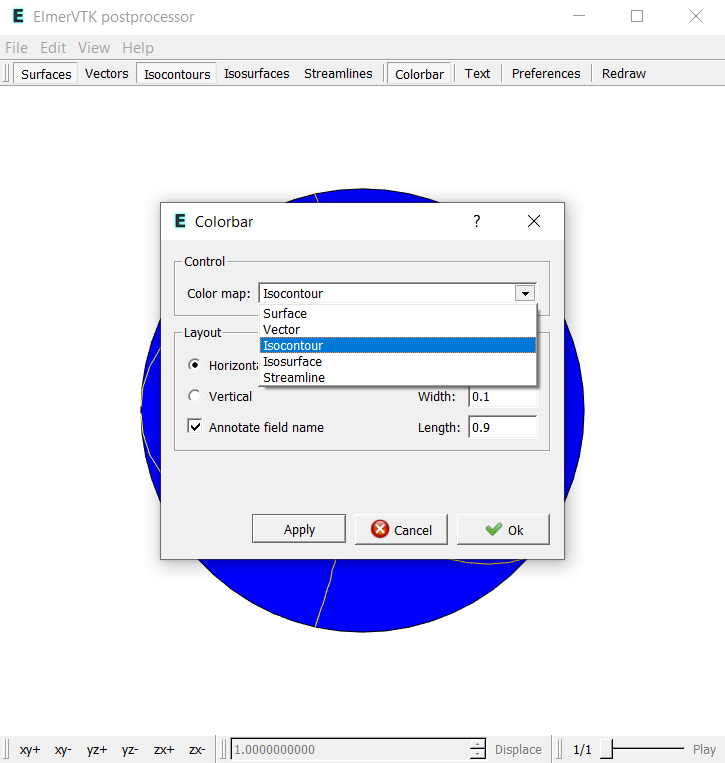
\includegraphics[width=0.48\textwidth]{vtk-6}
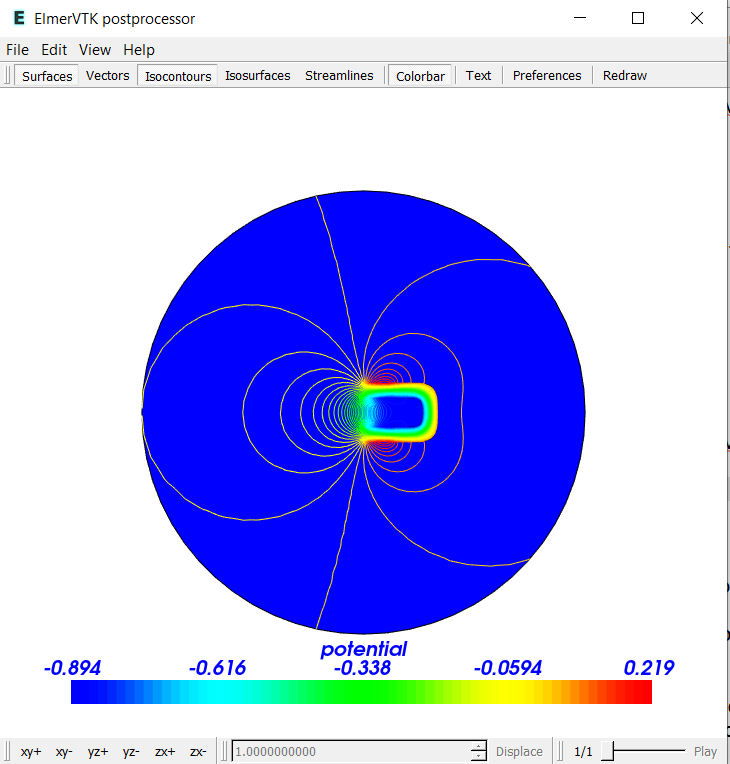
\includegraphics[width=0.48\textwidth]{vtk-7}
\caption{Add a Color Bar}\label{fg:vtk-6}
\end{center}
\end{figure}

We used a 2D example, so the choice of Isocontours made sense.  If we had used a 3D example, like the first heat tutorial, then Isosurfaces would make more sense.\\

As promised, ElmerVTK is fairly simple to use, and will make some pretty nice graphics in a short amount of time.

\chapter{Linux}

The Elmer website has instructions showing how to download binaries.\\

 \url{https://www.csc.fi/web/elmer/binaries}\\

Notice the section about using Launchpad Ubuntu and Debian based systems, as shown in Figure~\ref{fg:binaries}:\\

\begin{figure}[H]
\begin{center}
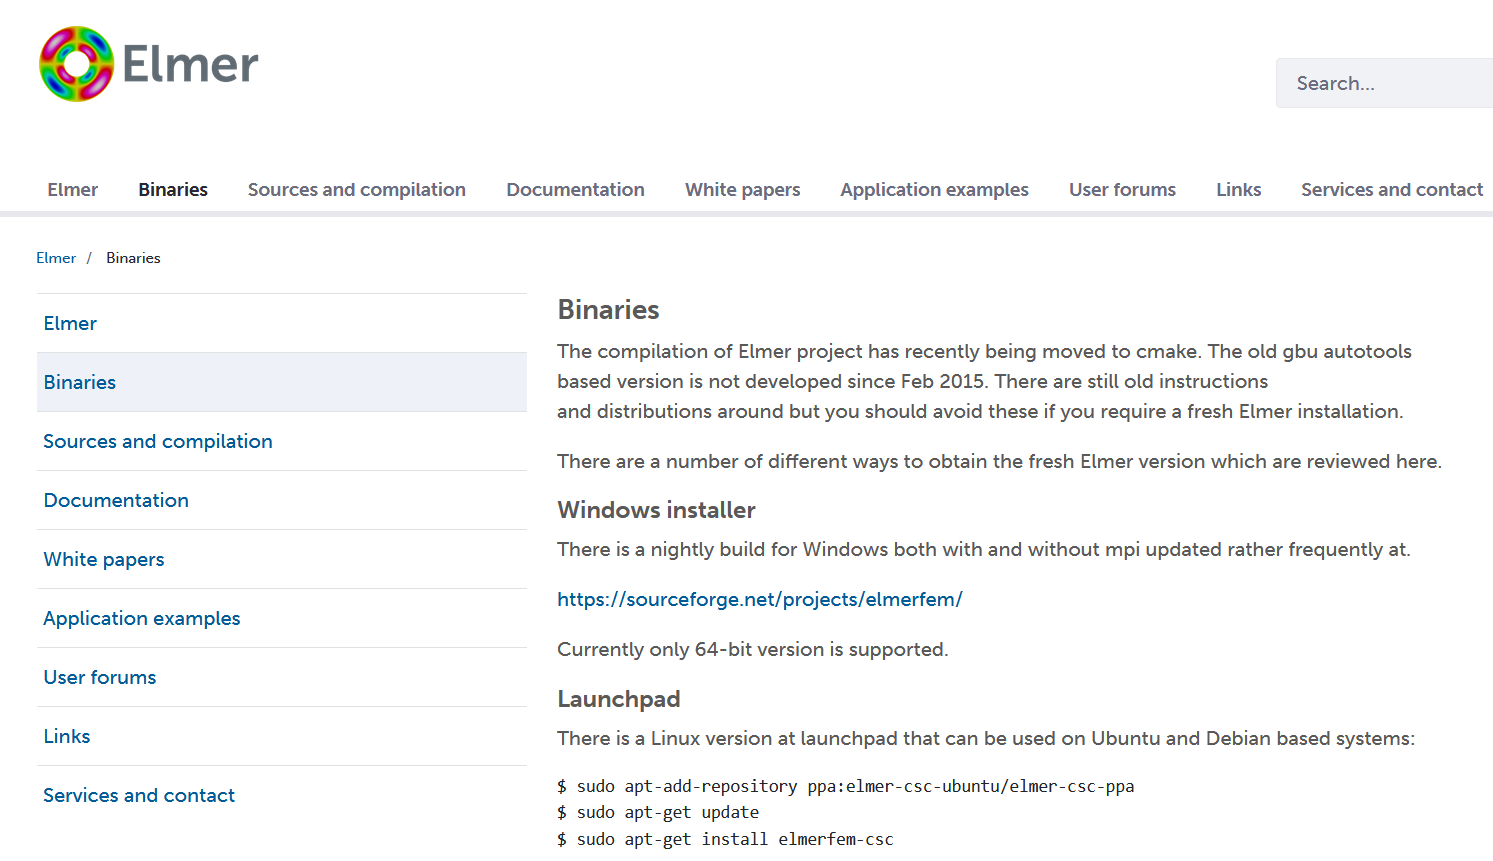
\includegraphics[width=0.8\textwidth]{binaries}
\caption{www.csc.fi/web/elmer/binaries}\label{fg:binaries}
\end{center}
\end{figure}


\texttt{sudo apt-add-repository ppa:elmer-csc-ubuntu/elmer-csc-ppa}

\texttt{sudo apt-get update}

\texttt{sudo apt-get install elmerfem-csc}

\texttt{sudo apt-get install elmerfem-csc-eg}\\

To start ElmerGrid and ElmerSolver, enter this in a terminal window:\\

\texttt{/bin/ElmerGrid}

\texttt{/bin/ElmerSolver}\\

To run ElmerGUI, enter this in a terminal window:\\

\texttt{/bin/ElmerGUI}\\

Next, install Paraview:\\

\texttt{sudo apt-get update}

\texttt{sudo apt-get install paraview}\\

Start ElmerGUI, run the first tutorial, and start Paraview from within ElmerGUI, by clicking on `Run', then `Start Paraview'.

\chapter{Virtual machine}

The Elmer website has instructions showing how to download a virtual machine.\\

 \url{http://www.nic.funet.fi/pub/sci/physics/elmer/bin/VirtualMachines}\\

Open that link, and there will be a directory with a few entries, as shown in Figure~\ref{fg:virt-1}.  Download two files, `Readme1st.txt' and  `CSC Ubuntu20 Elmer.ova'.  The .ova file is about 4 GB, so don't try this over dial-up!\\

\begin{figure}[H]
\begin{center}
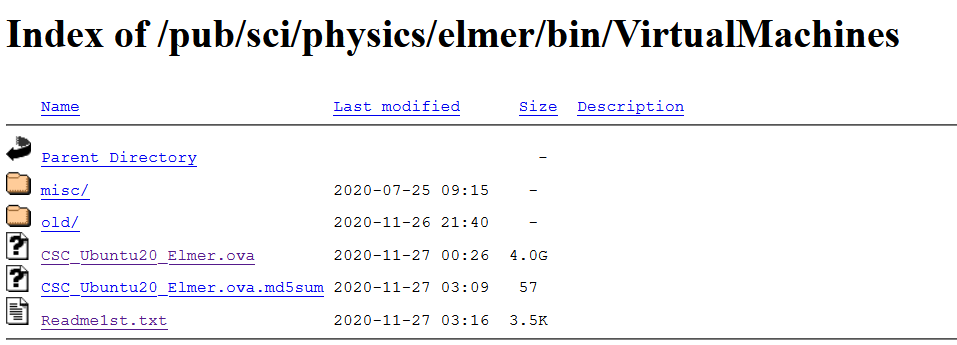
\includegraphics[width=0.8\textwidth]{virt-1}
\caption{www.csc.fi/web/elmer/bin/VirtualMachines}\label{fg:virt-1}
\end{center}
\end{figure}

Create an appropriate folder, such as `Elmer/VirtualMachine', and copy both files into that folder.  Open the file `Readme1st.txt', and follow the instructions for installing the .ova file in Virtual Box.  Open Import Appliance, as shown in Figure~\ref{fg:virt-2}.

\begin{figure}[H]
\begin{center}
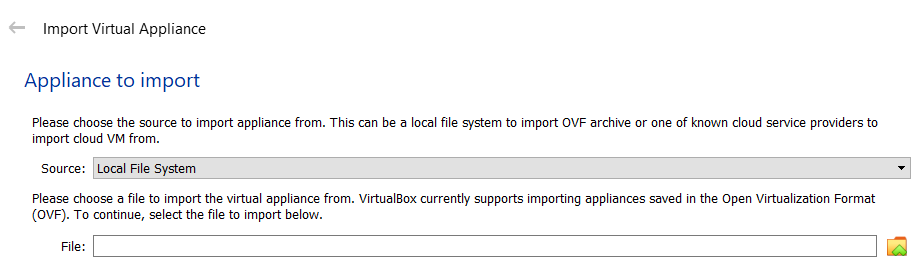
\includegraphics[width=0.8\textwidth]{virt-2}
\caption{Import Appliance}\label{fg:virt-2}
\end{center}
\end{figure}

Select the .ova file in the `Elmer/VirtualMachine' folder, as shown in Figure~\ref{fg:virt-3}. 

\begin{figure}[H]
\begin{center}
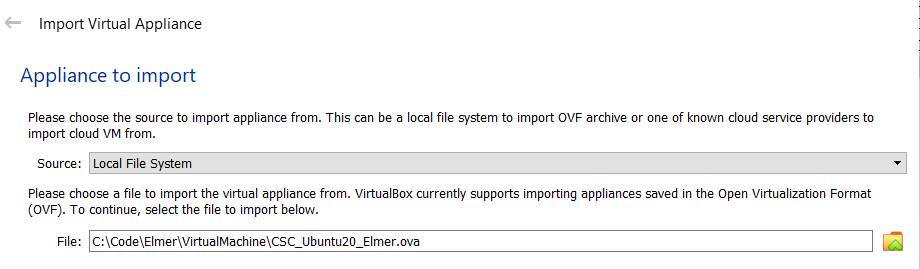
\includegraphics[width=0.8\textwidth]{virt-3}
\caption{Select the .ova file}\label{fg:virt-3}
\end{center}
\end{figure}

Click `Next' at the bottom of the screen.  The `Appliance settings' screen, as shown in Figure~\ref{fg:virt-4}, will open.  

\begin{figure}[H]
\begin{center}
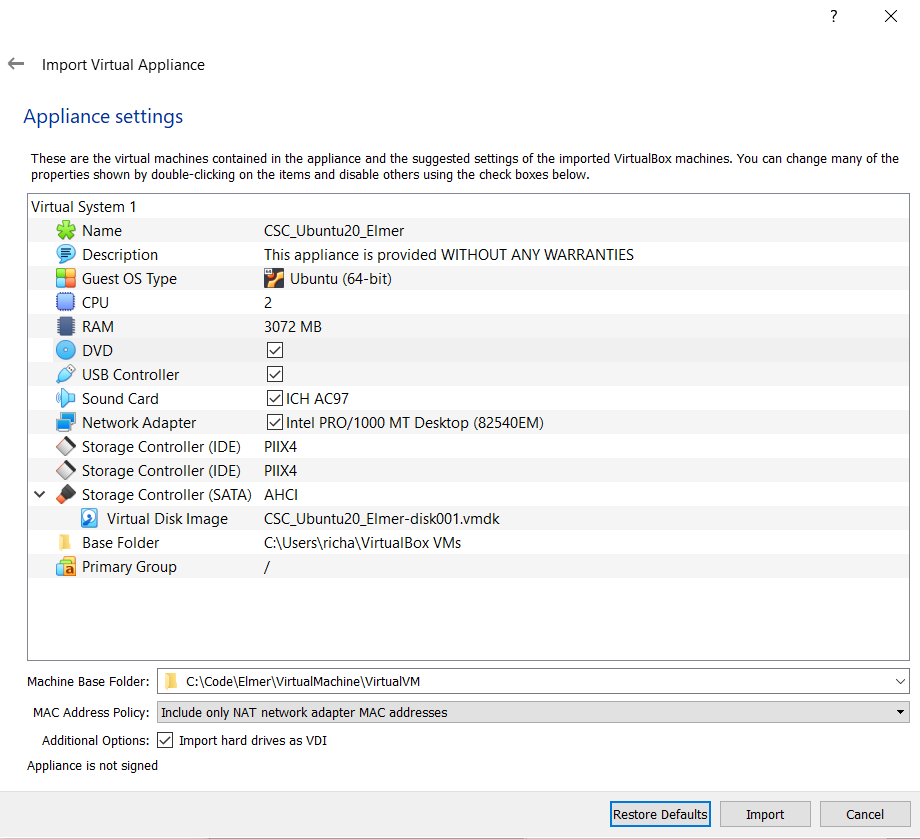
\includegraphics[width=0.8\textwidth]{virt-4}
\caption{Appliance settings}\label{fg:virt-4}
\end{center}
\end{figure}

Take the defaults for the settings.  The only (optional) exception to the defaults will be the `Machine Base Folder', which you may or may not want to change, so you can locate the VM right where you want it.  Also verify that you have enough installed RAM to match the default RAM setting of 3 GB.  When you are ready, click on `Import'.  Agree to the license agreement.  Importing the virtual disk image will take about five to ten minutes, depending on the speed of your hard drive, refer to Figure~\ref{fg:virt-5}.

\begin{figure}[H]
\begin{center}
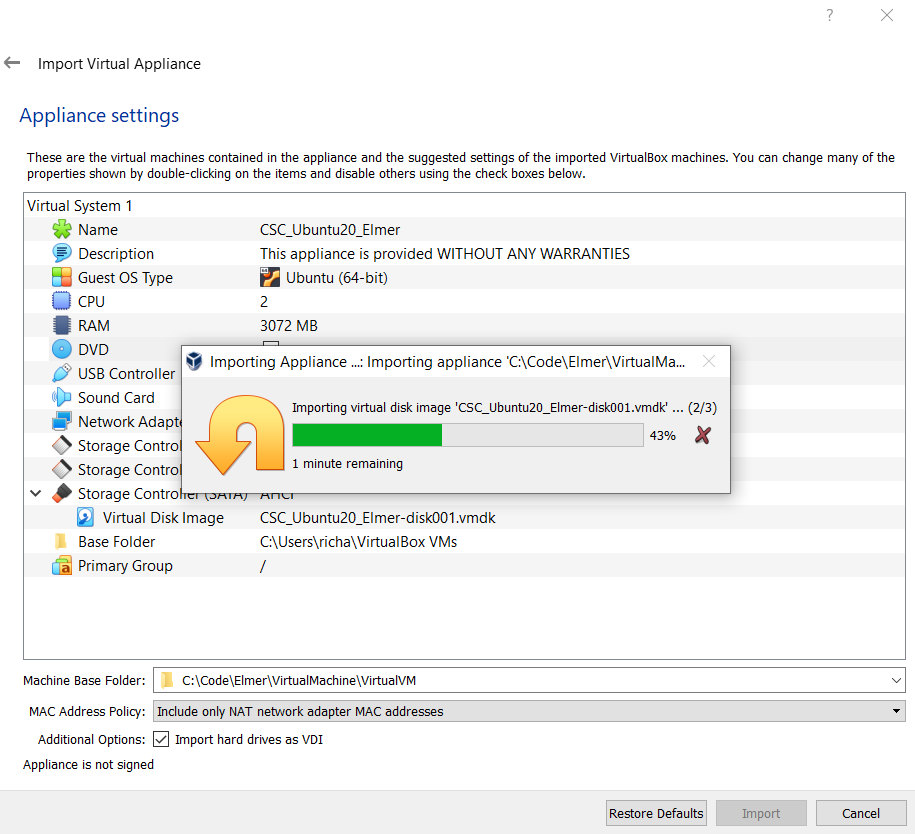
\includegraphics[width=0.75\textwidth]{virt-5}
\caption{Importing the virtual disk image}\label{fg:virt-5}
\end{center}
\end{figure}

Once Virtual Box is done importing the appliance, as usual with Virtual Box take a snapshot and then start the new virtual machine.  It should notify you that updated software needs to be downloaded, as shown in Figure~\ref{fg:virt-6}.

\begin{figure}[H]
\begin{center}
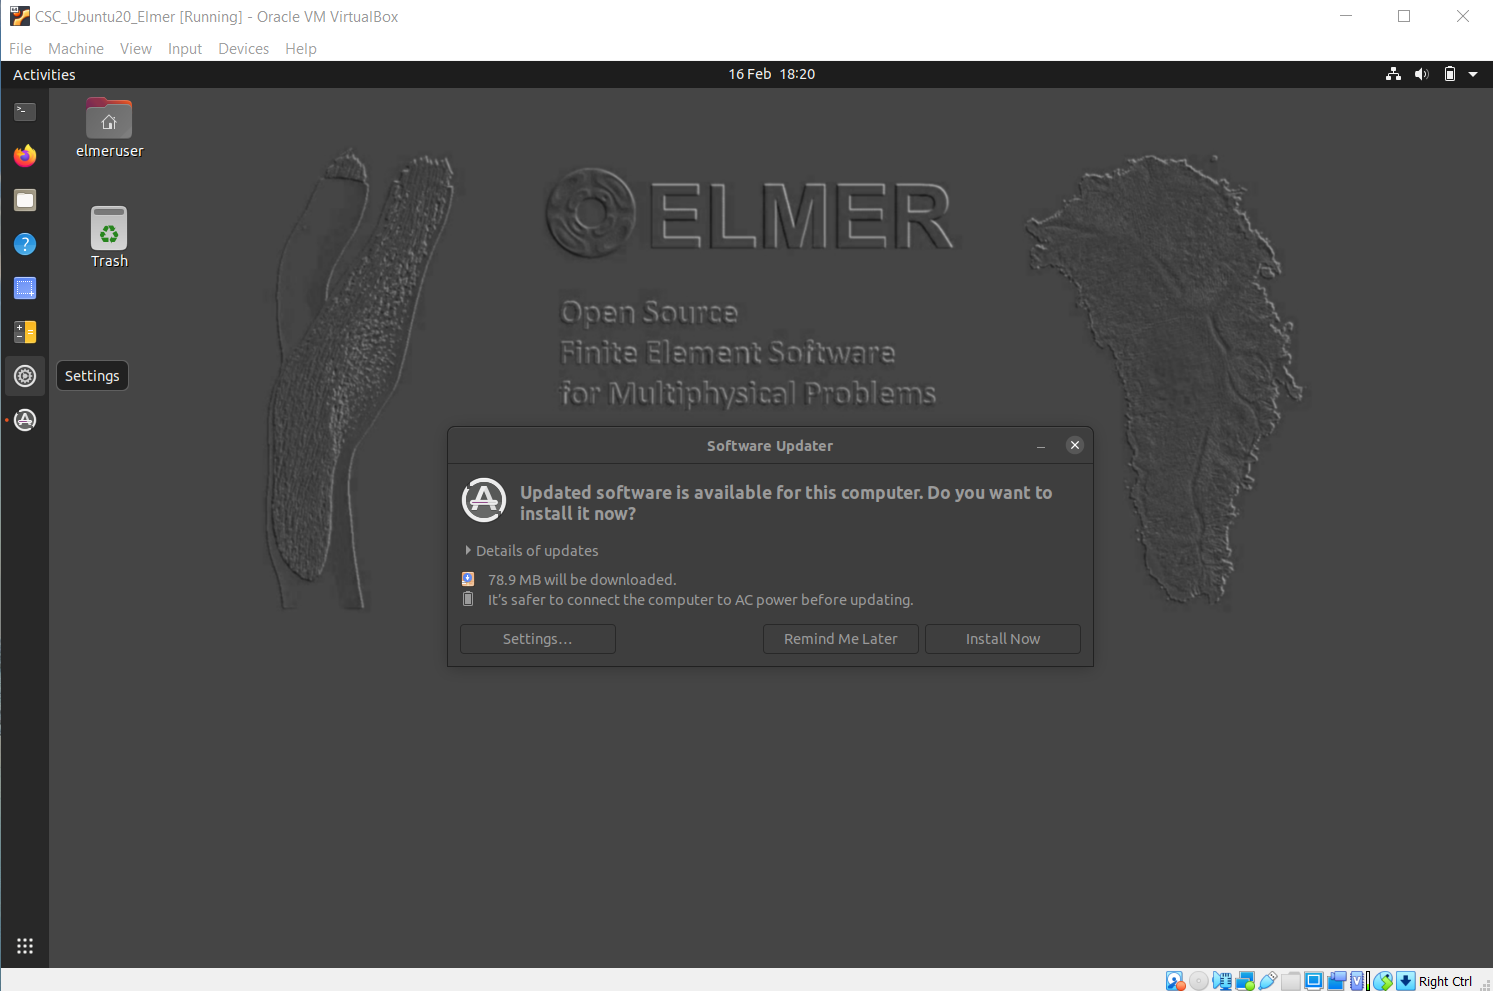
\includegraphics[width=0.8\textwidth]{virt-6}
\caption{Update software}\label{fg:virt-6}
\end{center}
\end{figure}

 Go ahead and update, when prompted, enter `elmerfem' to authenticate.  After updating is finished, it will restart once.  Shutdown and take another snapshot, now you have a fully updated Elmer Virtual Machine that you can always restore if needed.\\

One of many reasons to have an Elmer Virtual Machine is that now it is easy to compile ElmerSolver, ElmerGrid, and ElmerGUI, because all of the dependencies are included in the VM.










